\documentclass[pdftex,12pt,a4paper]{article}

\usepackage{graphicx}  
\usepackage[margin=2.5cm]{geometry}
\usepackage{breakcites}
\usepackage{indentfirst}
\usepackage{pgfgantt}
\usepackage{pdflscape}
\usepackage{float}
\usepackage{epsfig}
\usepackage{epstopdf}
\usepackage[cmex10]{amsmath}
\usepackage{stfloats}
\usepackage{multirow}

\renewcommand{\refname}{REFERENCES}
\linespread{1.3}

\usepackage{mathtools}
%\newcommand{\HRule}{\rule{\linewidth}{0.5mm}}
\thispagestyle{empty}
\begin{document}
\begin{titlepage}
\begin{center}
\textbf{}\\
\textbf{\Large{ISTANBUL TECHNICAL UNIVERSITY}}\\
\vspace{0.5cm}
\textbf{\Large{COMPUTER ENGINEERING DEPARTMENT}}\\
\vspace{2cm}
\textbf{\Large{BLG 242E\\ DIGITAL CIRCUITS LABORATORY\\ EXPERIMENT REPORT}}\\
\vspace{2.8cm}
\begin{table}[ht]
\centering
\Large{
\begin{tabular}{lcl}
\textbf{EXPERIMENT NO}  & : & 2 \\
\textbf{EXPERIMENT DATE}  & : & 21.02.2020 \\
\textbf{LAB SESSION}  & : & FRIDAY - 08.30 \\
\textbf{GROUP NO}  & : & G6 \\
\end{tabular}}
\end{table}
\vspace{1cm}
\textbf{\Large{GROUP MEMBERS:}}\\
\begin{table}[ht]
\centering
\Large{
\begin{tabular}{rcl}
150170087  & : & Sırrı Batuhan ÇOKSAK \\
150170039  & : & Fatih MURAT \\
\end{tabular}}
\end{table}
\vspace{2.8cm}
\textbf{\Large{SPRING 2020}}

\end{center}
\end{titlepage}

\thispagestyle{empty}
\addtocontents{toc}{\contentsline {section}{\numberline {}FRONT COVER}{}}
\addtocontents{toc}{\contentsline {section}{\numberline {}CONTENTS}{}}
\setcounter{tocdepth}{4}
\tableofcontents
\clearpage

\setcounter{page}{1}

\section{INTRODUCTION}

In this experiment we were tasked with several objectives which include designing and implementing digital circuits of expressions, finding dual of a theorem also validating it, taking the complement of an expression and implementing it and checking our results, and simplifying a logical function also implementing the simplified version. 

\section{MATERIALS AND EXPERIMENT}

\subsection{PART 1}
In the first part of the experiment we were expected to design and implement logic circuits for the given two expressions, which are
\begin{itemize}
    \item $F_{1}(a,b) = a + a . b$
    \item $F_{2}(a,b) = (a + b) . (a + b')$
\end{itemize}
We used integrated circuits 74xx04 (Hex Inverters), 74xx08  ( Quadruple 2-input Positive AND Gates ) and 74xx32 ( Quadruple 2-input Positive OR Gates ) when needed.

First expression can be simplified, and the result can be used to validate the circuit design. The simplification is as follows:
\begin{align}
F_{1}(a,b) &= a + a . b\notag\\ 
&= a . ( 1 + b ) \tag{Distribution} \\
&= a . ( 1 ) \tag{Annihilation} \\
&= a \tag{Identity} \\
\notag \end{align}

Simplification also proves absorption theorem since $F_{1}$ is in that form, using the $F_{1}$ and the result from simplification we created the following truth table.

\begin{table}[H]
\centering
\begin{tabular}{|c|c|c|c|c|}
\hline
a & b & (a.b) & a+(a.b)  & a      \\ \hline
0 & 0 & 0 & 0       & 0        \\ 
0 & 1 & 0 & 0       & 0        \\ 
1 & 0 & 0 & 1       & 1        \\ 
1 & 1 & 1 & 1       & 1        \\  \hline
\end{tabular}
\caption{Truth table of the $F_{1}$ (also absorption theorem)}
\label{Table 1}
\end{table}
\clearpage
After creating the truth table, we analyzed $F_{1}$ using our knowledge of logic gates we designed the digital circuit design in the following figure.

\begin{figure}[H]
	\centering
	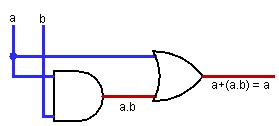
\includegraphics[width=0.5\textwidth]{E2P1.1.1.jpg}
	\caption{Circuit design of $F_{1}$}
	\label{Figure 1}
\end{figure}

After designing the digital circuit of $F_{1}$ we started implementing the circuit, We connected inputs to logic switches, output to a LED. Also when design required an and gate we used IC 74xx08 and when it required an or gate we used IC 74xx32. Following figure shows the 4 different state that this circuit can be, light green color in LED shows low voltage value (0) and red shows high (1).

\begin{figure}[H]
	\centering
	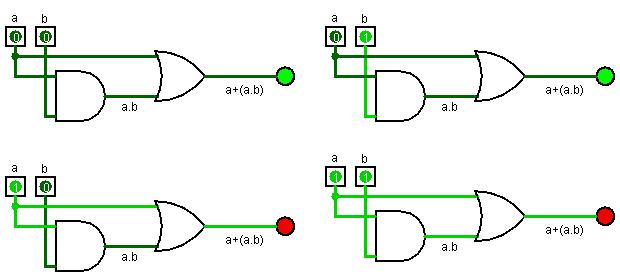
\includegraphics[width=1\textwidth]{E2P1.1.2.jpg}
	\caption{}
	\label{Figure 2}
\end{figure}

Additionally figure 2 can be used for validation of the circuit. From the simplification of $F_{1}$ we found that the output is equal to $a$ and Figure 2 also validates it. 

\clearpage
Second expression can be simplified, and the result can be used to validate the circuit design. The simplification operation is:
\begin{align}
F_{2}(a,b) &= (a + b) . (a + b')\notag\\ 
&= a + ( b + b' ) \tag{Distribution} \\
&= a + ( 0 ) \tag{Inverse} \\
&= a \tag{Identity} \\
\notag \end{align}

Using the $F_{2}$ and the result from simplification we created the following truth table.

\begin{table}[H]
\centering
\begin{tabular}{|c|c|c|c|c|c|c|}
\hline
a & b & b' & a+b  &(a+b')  &(a+b).(a+b') &a \\ \hline
0 & 0 & 1 & 0       & 1       & 0   & 0 \\ 
0 & 1 & 0 & 1       & 0       & 0   & 0 \\ 
1 & 0 & 1 & 1       & 1       & 1   & 1 \\ 
1 & 1 & 0 & 1       & 1       & 1   & 1 \\  \hline
\end{tabular}
\caption{Truth table of the $F_{2}$}
\label{Table 2}
\end{table}

After creating the truth table, we analyzed $F_{2}$ using our knowledge of logic gates we designed the digital circuit design in the following figure.

\begin{figure}[H]
	\centering
	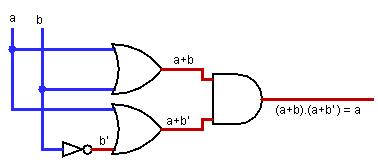
\includegraphics[width=0.6\textwidth]{E2P1.2.1.jpg}
	\caption{Circuit design of $F_{2}$}
	\label{Figure 3}
\end{figure}

After designing the digital circuit of $F_{2}$ we started implementing the circuit, We connected inputs to logic switches, output to a LED. Also when design required an and gate we used IC 74xx08, when it required an or gate we used IC 74xx32and when it required an not gate we used IC 74xx04. Following figure shows the 4 different state that this circuit can be, light green color in LED shows low voltage value (0) and red shows high (1).

\begin{figure}[H]
	\centering
	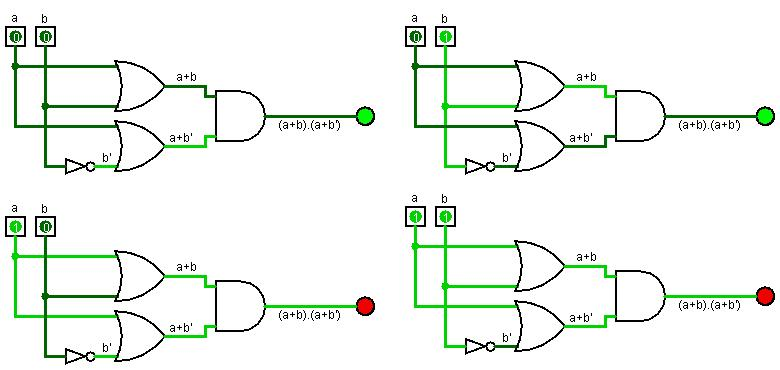
\includegraphics[width=1\textwidth]{E2P1.2.2.jpg}
	\caption{}
	\label{Figure 4}
\end{figure}

Additionally figure 4 can be used for validation of the circuit. From the simplification of $F_{2}$ we found that the output is equal to $a$ and Figure 4 also validates it. 

\subsection{PART 2}
In this part of the experiment we were tasked with determining the dual of the given theorem and implementing the theorem using logic gates. We used integrated circuits 74xx08 ( Quadruple 2-input Positive AND Gates ) and 74xx32 ( Quadruple 2-input Positive OR Gates ) in this part of the experiment.
Given theorem is: $a + a.b = a$ . It should be noted that when taking the dual of the theorem, it should be considered as: $ a + (a.b) = a $. To find a dual of a theorem we changed "."s to "+" and "+"s to ".", but keep the variables and the parenthesises.
\newline
Dual of the theorem is $a.(a+b) = a$. Using the dual of the theorem we created the following truth table.

\begin{table}[H]
\centering
\begin{tabular}{|c|c|c|c|c|}
\hline
a & b & (a+b) & a.(a+b)  & a      \\ \hline
0 & 0 & 0 & 0       & 0        \\ 
0 & 1 & 0 & 0       & 0        \\ 
1 & 0 & 1 & 1       & 1        \\ 
1 & 1 & 1 & 1       & 1        \\  \hline
\end{tabular}
\caption{Truth table of the dual of the given theorem}
\label{Table 3}
\end{table}

After creating the truth table, we analyzed the dual of the given theorem and using our knowledge of logic gates we designed the digital circuit design in the following figure

\begin{figure}[H]
	\centering
	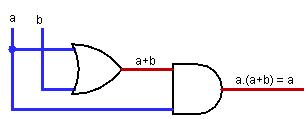
\includegraphics[width=0.5\textwidth]{E2P2.1.1.jpg}
	\caption{Circuit design of the dual of the given theorem}
	\label{Figure 5}
\end{figure}

After designing the digital circuit, we started implementing the circuit, We connected inputs to logic switches, output to a LED. Also when design required an and gate we used IC 74xx08 and when it required an or gate we used IC 74xx32. Following figure shows the 4 different state that this circuit can be, light green color in LED shows low voltage value (0) and red shows high (1). Additionally for the right side of the expression we connected the input $a$ to a LED.  

\begin{figure}[H]
	\centering
	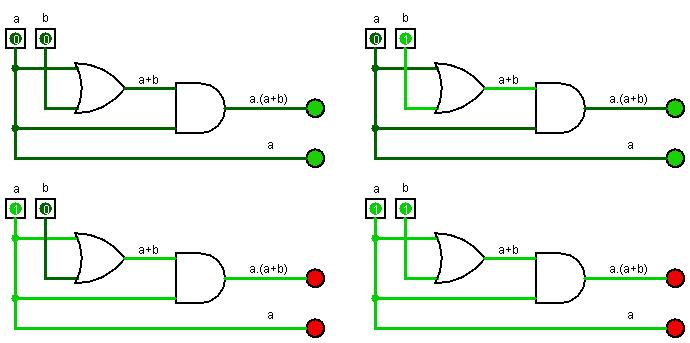
\includegraphics[width=1\textwidth]{E2P2.1.2.jpg}
	\caption{}
	\label{Figure 6}
\end{figure}
From figure 6 it is clear that the left side expression of the dual of the given theorem (which is $a + (a.b)$) is same the right side expression ( $a$ ). Hence, figure validates that our design and implementation also the operation of taking dual of a theorem.
\clearpage
\subsection{PART 3}
\paragraph{}
In the third part of the experiment, we were asked to find the complement of the given expression below, implement the proper digital circuit for it and validate it using the truth table.
\begin{itemize}
    \item $F_{3}$(a,b,c) = ($a \cdot b$) + ($a' \cdot b$)
\end{itemize}
\paragraph{}
In order to find the complement of the given expression, we replaced input variables with their inverses, AND signs with OR signs and OR signs with AND signs. As a result, we obtained the expression below;
\begin{itemize}
    \item $F'_{3}$(a,b,c) = $(a'+b') \cdot (a+c')$
\end{itemize}
With taking the complement of the given expression, we created the truth table for $F'_{3}$.

\begin{table}[h]
\centering
\begin{tabular}{|c|c|c|c|c|c|c|c|c|}
\hline
a & b & c & a' & b' & c' & a'+ b' & a + c' & $F'_{3}$ = $(a' + b') \cdot (a + c')$ \\ \hline
0 & 0 & 0 & 1  & 1  & 1     & 1      & 1             & 1        \\ 
0 & 0 & 1 & 1  & 1  & 0     & 1      & 0             & 0        \\ 
0 & 1 & 0 & 1  & 0  & 1     & 1      & 1             & 1        \\ 
0 & 1 & 1 & 1  & 0  & 0     & 1      & 0             & 0        \\ 
1 & 0 & 0 & 0  & 1  & 1     & 1      & 1             & 1        \\ 
1 & 0 & 1 & 0  & 1  & 0     & 1      & 1             & 1        \\
1 & 1 & 0 & 0  & 0  & 1     & 0      & 1             & 0        \\ 
1 & 1 & 1 & 0  & 0  & 0     & 0      & 1             & 0        \\ \hline
\end{tabular}
\caption{Truth table for $F'_{3}$}
\label{Table 4}
\end{table}

\clearpage
\paragraph{}
Using an OR gate, 2 AND gates and 3 inverters, we implemented our complemented expression as Figure 7 shows.

\begin{figure}[!h]
	\centering
	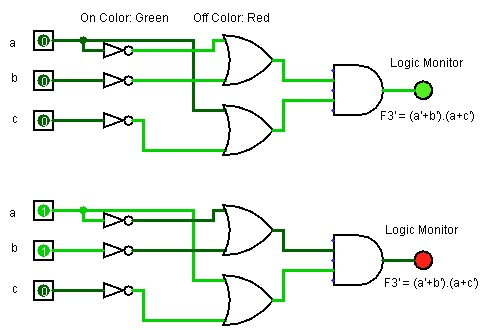
\includegraphics[width=0.5\textwidth]{E2P3.1.1.jpg}	
	\caption{Circuit for complement of F3}
	\label{Figure 7}
\end{figure}

\paragraph{}
In detail, while implementing our circuit we used 74000 series ICs below;
\begin{itemize}
    \item 74xx04 - Hex Inverters
    \item 74xx08 - Quadruple 2-input Positive AND Gates
    \item 74xx32 - Quadruple 2-input Positive OR Gates
\end{itemize}

\paragraph{}

Firstly, we give Vcc voltage to the top right corner pin and ground voltage to the bottom left corner pin of all of the ICs used in the implementetion.

\paragraph{}

After we applied the supply voltage, we used 6 pins of the inverter. Connecting first input(a) to the thirteenth pin of the inverter, we obtained complement of the first input from twelfth pin of the inverter; connecting second input(b) to the eleventh pin of the inverter, we obtained complement of the second input from tenth pin of the inverter; connecting third input(c) to the ninth pin of the inverter, we obtained complement of the third input from the eighth pin of the inverter.

\paragraph{}

After we obtained the all smallest necessary elements, we connected them into the OR gate. Connecting twelfth pin of the inverter to the thirteenth pin of the OR gate and tenth pin of the inverter to the twelfth pin of the OR gate, we obtained (a'+b') from the eleventh pin of OR gate; connecting first input directly from the switch to the tenth pin of the OR gate and connecting eighth pin of the inverter to the ninth pin of the OR gate, we obtained (a+c') from the eighth of the OR gate.

\paragraph{}

After we are done with the OR gate, we used AND gate to get final expression. Connecting elevent pin of the OR gate to the thirteenth pin of the AND gate and  connecting eighth pin of the OR gate to the twelfth pin of the AND gate, we obtained (a'+b').(a+c') from eleventh pin of the AND gate.

\paragraph{}

After we are done with the ICs, we connected our final expression from the eleventh pin of the AND gate to the LED monitor. In the end, we played with the input values and observed the output values. Results were verified by out truth table and there was no mistake.

\clearpage



\subsection{PART 4}

\paragraph{}
In the fourth and last part of the experiment, we are given set of 1-generating points;

\begin{itemize}
    \item $F_{4}$(a,b,c,d) = $U_{1}$(1,2,5,6,9,10,13,14)  
\end{itemize}

\paragraph{}
We can write down the augmented expression of $F_{4}$ from the given set of 1-generating points;\newline \newline
$F_{4}$(a,b,c,d) = (a'b'c'd) + (a'b'cd') + (a'bc'd) + (a'bcd') + (ab'c'd) + (ab'cd') + (abc'd) + (abc'd)

\paragraph{}
Using axioms of boolean algebra, we can simplfy $F_{4}$ as follows;

\begin{align}
F_{4}(a,b,c,d) &= (a'b'c'd) + (a'b'cd') + (a'bc'd) + (a'bcd') + (ab'c'd) + (ab'cd') + (abc'd) + (abc'd) \notag\\ 
&= (a b' c' d) + (abc'd) + (a'b'cd') + (a'bcd') + (a'   b'   c'   d) + (a'   b   c'   d) + (a   b'   c   d') + (a   b   c   d') \tag{Commutativity} \\
&= ac'd(b' + b) + a'cd'(b'+b) + a'c'd(b' + b) + acd'(b'+b) \tag{Distribution} \\
&= ac'd(1) + a'cd'(1) + a'c'd(1) + acd'(1) \tag{Inverse} \\
&= ac'd + a'cd'+ a'c'd+ acd' \tag{Identitiy} \\
&= ac'd + a'c'd + a'cd' + acd' \tag{Commutativity} \\
&= c'd(a + a') + cd'(a' + a) \tag{Distribution} \\
&= c'd(1) + cd'(1) \tag{Inverse} \\
F_{4}(a,b,c,d) &= c'd + cd'(XOR) \tag{Identity} \\
\notag \end{align}

\clearpage

\paragraph{}
After we simplified the expression, it is obvious that simplified form of $F_{4}$ is equal to XOR of c and d in terms of output results. Using basic knowledge from the digital circuit course, we can easily create the truth table for simplified $F_{4}$ as follows; \newline \newline \newline

\begin{table}[h]
\centering
\begin{tabular}{|c|c|c|c|c|c|c|c|c|}
\hline
a & b & c & d & c' & d' & $c' \cdot d$ & $c \cdot d'$ & $F_{4}$ = $c' \cdot d$ + $c \cdot d'$ \\ \hline
0 & 0 & 0 & 0 & 1  & 1  & 0      & 0      & 0                    \\ \hline
0 & 0 & 0 & 1 & 1  & 0  & 1      & 0      & 1                    \\ \hline
0 & 0 & 1 & 0 & 0  & 1  & 0      & 1      & 1                    \\ \hline
0 & 0 & 1 & 1 & 0  & 0  & 0      & 0      & 0                    \\ \hline
0 & 1 & 0 & 0 & 1  & 1  & 0      & 0      & 0                    \\ \hline
0 & 1 & 0 & 1 & 1  & 0  & 1      & 0      & 1                    \\ \hline
0 & 1 & 1 & 0 & 0  & 1  & 0      & 1      & 1                    \\ \hline
0 & 1 & 1 & 1 & 0  & 0  & 0      & 0      & 0                    \\ \hline
1 & 0 & 0 & 0 & 1  & 1  & 0      & 0      & 0                    \\ \hline
1 & 0 & 0 & 1 & 1  & 0  & 1      & 0      & 1                    \\ \hline
1 & 0 & 1 & 0 & 0  & 1  & 0      & 1      & 1                    \\ \hline
1 & 0 & 1 & 1 & 0  & 0  & 0      & 0      & 0                    \\ \hline
1 & 1 & 0 & 0 & 1  & 1  & 0      & 0      & 0                    \\ \hline
1 & 1 & 0 & 1 & 1  & 0  & 1      & 0      & 1                    \\ \hline
1 & 1 & 1 & 0 & 0  & 1  & 0      & 1      & 1                    \\ \hline
1 & 1 & 1 & 1 & 0  & 0  & 0      & 0      & 0                    \\ \hline
\end{tabular}
\caption{Truth table for simplified $F_{4}$}
\label{Table 5}
\end{table}
\clearpage

\paragraph{}
After we simplified the expression, we implemented our circuit. Figure 8 shows our circuit implementation.

\begin{figure}[!h]
	\centering
	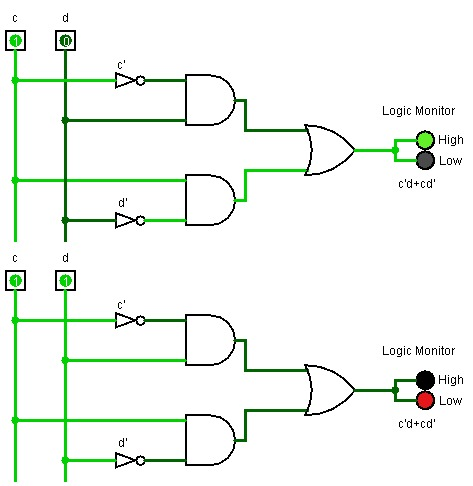
\includegraphics[width=0.5\textwidth]{E2P4.1.1.jpg}	
	\caption{Example states for simplified $F_{4}$}
	\label{Figure 8}
\end{figure}

\paragraph{}
Connecting first input(c) directly from switch to thirteenth pin of the inverter, we obtained complement of first input from the twelfth pin of the inverter; connecting second input(d) directly from switch to eleventh pin of the inverter, we obtained complement of second input from the tenth pin of the inverter.
\paragraph{}
Connecting twelfth pin of the inverter to thirteenth pin of the AND gate and connecting second input directly from the switch to the twelfth pin of the AND gate, we obtained (c'd) from eleventh pin of the AND gate; connecting first input directly from the switch to the tenth pin of the AND gate and connecting tenth pin of the inverter to the ninth pin of the AND gate, we obtained (cd') from eighth pin of the AND gate. 
\paragraph{}
Connecting eleventh pin of the AND gate to thirteenth pin of the OR gate and connecting eighth pin of the AND gate to the twelfth pin of the OR gate, we obtained the final expression which is c'd + cd' from the eleventh pin of the OR gate. In the end, we connected eleventh pin of the OR gate(final expression) to the LED monitor and playing with the input values, we observed the output results. There was no mistake and truth table verified our circuit implementation.

\subsection{EQUIPMENT USED}
\begin{itemize}
    \item C.A.D.E.T
    \item 74xx04 - Hex Inverters
    \item 74xx08 - Quadruple 2-input Positive AND Gates
    \item 74xx32 - Quadruple 2-input Positive OR Gates
\end{itemize}

\clearpage
\section{RESULTS}
Throughout the whole experiment the results we obtained was not different from the expected results which we calculated before the implementation of the functions and expressions. Since the equipment we used during the experiment were mostly integrated circuits results were output values of these equipment and the results was certain either one or zero. Hence, we obtained precise results and verified our results using truth tables.


\section{DISCUSSION}
During the preparation phase of the experiment parts we did the necessary objectives such as simplification of an expression or creating a truth table individually so that our individual skills in these areas can improve, later we checked our results by comparing however, during the design phase of the parts we analyzed the expression which we will implement, decided which integrated circuits we will use, and planned their position on the breadboard so that cables look more organized and easy to follow ( for example we decided not to use more than 2 ICs in a vertical position since it would result with a lot of cables going vertically which is hard to trace). During the implementation we followed our design in the design phase and completed the implementation. Last part was checking if our design and implementation was correct, as stated in the "RESULTS" section implementation results was same with the expected results from the preparation phase for every part hence; we managed to complete parts rather quickly.

\section{CONCLUSION}
We managed to finish experiment without any major setbacks however, there were minor one which costs us few minutes. We did not color code the cables of inputs and outputs at some point in part 4 we lost track of our cables and we had to retrace them. We decided to be more careful about this issue in the future by color coding the cables we will be using. Overall experiment helped us getting more comfortable at using integrated circuits, designing digital circuits and doing Boolean algebra operations.


\newpage
\nocite{*}
\addcontentsline{toc}{section}{\numberline {}REFERENCES}

\bibliographystyle{unsrt}
\bibliography{reference}

\end{document}

